\usetikzlibrary{patterns}

\section{Resumen de }
\subsection{Electrostatica y Magnetostatica}

Se comenzara analizando los campos electros y magneticos cuando estos son estaticos, es decir, no varian en el tiempo. Para ello, se considera el vacio, es decir, no hay materia en el espacio. 
\begin{equation}
    \begin{array}{c|c}
    \textbf{Vacío (diferencial)} & \textbf{Vacío (integral)} \\[8pt]
    \nabla \cdot \mathbf{E} = \frac{1}{\varepsilon_0} \rho 
    & \oint \mathbf{E} \cdot d\mathbf{a} = \frac{1}{\varepsilon_0} \int \rho \, d\tau \\[5pt]
    \nabla \cdot \mathbf{B} = 0 
    & \oint \mathbf{B} \cdot d\mathbf{a} = 0 \\[5pt]
    \nabla \times \mathbf{E} = 0 
    & \oint \mathbf{E} \cdot d\mathbf{l} = 0 \\[5pt]
    \nabla \times \mathbf{B} = \mu_0 \mathbf{J} 
    & \oint \mathbf{B} \cdot d\mathbf{l} = \mu_0 \int \mathbf{J} \cdot d\mathbf{a}
    \end{array}
\end{equation}
Dado que el campo electrico es conservativo, se puede definir un potencial escalar $\phi$ tal que $\mathbf{E} = -\nabla \phi$. Lo que permite derivar la \textbf{ecuacion de Poisson} dada por:
\begin{align}
    \nabla^2 \phi = -\frac{\rho}{\varepsilon_0}
\end{align}
Donde se define $\phi$ como el potencial escalar electrico, $\rho$ como la densidad de carga (La cual corresponde a la suma de carga libre y carga ligada) y $\varepsilon_0$ como la permitividad del vacio. En la mayor parte de los casos se tendra que la densidad de carga sera nula(debido a los medios) que da como resultado la ecuacion de Laplace
\begin{align}
    \nabla^2 \phi = 0
\end{align}
Donde este potencial quedara sujeto a la geometria y coordenadas de cada problema.Este potencial presenta propiedades importantes:
\begin{itemize}
    \item El potencial posee solo una solución y es única.
    \item El potencial no tolera mínimos ni máximos locales, y el valor en cierto punto del espacio es el promedio de los valores en la frontera.
    \item La solución es una función armónica.
    \item La ecuación cumple con la condición de linealidad.
\end{itemize}
Las condiciones de borde corresponden a las condiciones que se deben cumplir en la frontera de un sistema, estas condiciones vienen dadas por:
\begin{equation}
    \begin{array}{c|c}
    \textbf{Condiciones de borde eléctricas} & \textbf{Condiciones de borde magnéticas} \\[8pt]
    E_{t1} - E_{t2} = 0 & (H_{t1} - H_{t2}) = J_s \\[10pt]
    \hat{n} \cdot (\vec{D}_1 - \vec{D}_2) = \rho_s & \hat{n} \cdot (\vec{B}_{n1} - \vec{B}_{n2}) = 0
    \end{array}
\end{equation}
Para el caso de un conductor perfecto es decir $\sigma = \infty$ se tendran las siguientes condiciones de borde:
\begin{equation}
    \begin{array}{c c}
        E_t = 0 \quad\quad\quad\quad & \hat{n} \times \vec{E} = 0 \\[12pt]
        D_n = \rho_s \quad\quad\quad\quad & \hat{n} \cdot \vec{D} = \rho_s \\[12pt]
        B_n = 0 \quad\quad\quad\quad & \hat{n} \cdot \vec{B} = 0 \\[12pt]
        H_t = J_s \quad\quad\quad\quad & \hat{n} \times \vec{H} = \vec{J}_s
    \end{array}
\end{equation}
Donde para la mayoria de casos de resolucion se tendra la corriente superficial ($J_s$) y la densidad de carga superficial ($\rho_s$) seran nulas.\\

Algunos consejos utiles para la resolucion de los problemas son:
\begin{itemize}
    \item Recordar las expresiones de los campos eléctricos, potenciales, cargas, etc. Vistos en Electromagnetismo
    \item Analizar la geometría del esquema y ver si es aplicable utilizar Laplace.
    \item Verificar qué tipo de coordenadas son más acordes al problema.
    \item Es fundamental analizar la dirección del potencial eléctrico, dado que este nos dará la respuesta a qué tipo de coordenada/s dependerá este.
    \item Ver cuántos medios dispone el problema y separar por escenarios cada uno de estos.
    \item Analizar el problema para obtener las ecuaciones que hagan falta para poder despejar las constantes que permitan obtener una expresión explícita del potencial o campo eléctrico.
    \item Ver si es posible aplicar condiciones de borde para el punto anterior.
\end{itemize}
\newpage
\subsection{Problema}
\begin{problema} %Problema 1
    Para la estructura coaxial de la Figura 1, de longitud \(d\) y diferencia de potencial \(V_{0}\) entre los electrodos en \(r = a\) y \(r = c\), determinar:
    \begin{enumerate}
        \item Potencial \(\phi(r)\) y campo \(E\) en los medios dieléctricos perfectos de permisividad \(\epsilon_{1}\) y \(\epsilon_{2}\).
        \item Carga total \(Q\) en cada uno de los electrodos (demuestre que la magnitud es igual). 
        \item Energía acumulada en campo \(E\) en cada medio dieléctrico.
    \end{enumerate}
    \begin{center}
        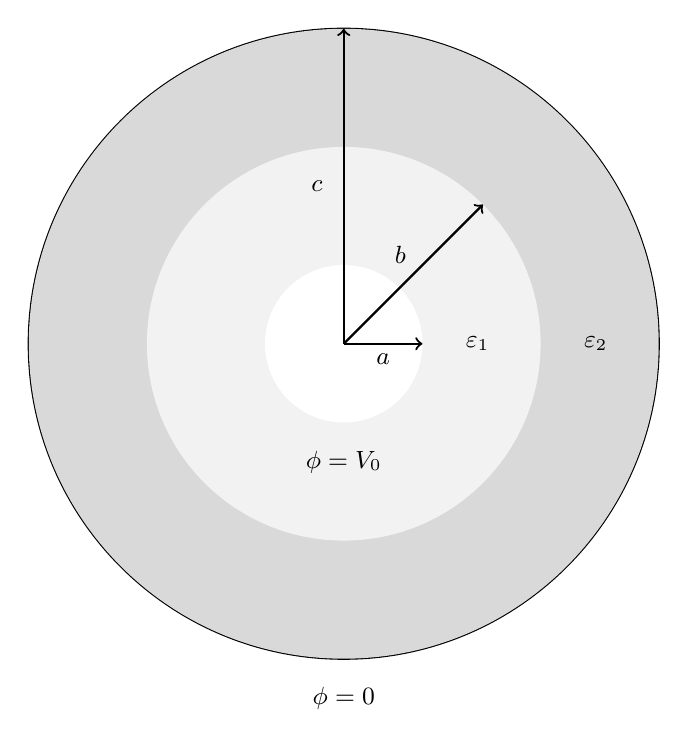
\begin{tikzpicture}
            % Definir los radios
            \def\ra{1}  % Radio interno
            \def\rb{2.5}    % Radio intermedio
            \def\rc{4}  % Radio externo
    
            % Dibujar los círculos
            \draw[thick, black] (0,0) circle (\ra);
            \draw[thick] (0,0) circle (\rb);
            \draw[thick] (0,0) circle (\rc);
    
            % Sombreado de la región externa
            \begin{scope}
                \clip (0,0) circle (\rc);
                \fill[gray!30] (-5,-5) rectangle (5,5);
            \end{scope}
        
            \begin{scope}
                \clip (0,0) circle (\rb);
                \fill[gray!10] (-5,-5) rectangle (5,5);
            \end{scope}
            
            \begin{scope}
                \clip (0,0) circle (\ra);
                \fill[white] (-5,-5) rectangle (5,5);
            \end{scope}

            % Flechas radiales
            \draw[thick,->] (0,0) -- (\ra,0) node[midway,below] {\small $a$};
            \draw[thick,->] (0,0) -- ({\rb*cos(45)},{\rb*sin(45)}) node[midway,above left,xshift=1pt] {\small $b$};
            \draw[thick,->] (0,0) -- ({\rc*cos(90)},{\rc*sin(90)}) node[midway,left,xshift=-4pt] {\small $c$};

    
            % Etiquetas de materiales
            \node at (\ra+0.7,0) {\small $\varepsilon_1$};
            \node at (\rb+0.7,0) {\small $\varepsilon_2$};
    
            % Condiciones de potencial
            \node at (0,-\ra-0.5) {\small $\phi = V_0$};
            \node at (0,-\rc-0.5) {\small $\phi = 0$};
    
        \end{tikzpicture}
    \end{center}
\end{problema}
\begin{proof} %Resolucion problema 1
    La resolucion viene dada por:
    \begin{enumerate}
        \item Se menciona en el problema que la geométrica corresponde a una esfera maciza y por tanto será conveniente el utilizar coordenadas esféricas (debido esto se observa que el campo eléctrico \textbf{V} solo depende de $\hat{\rho}$ y no de alguna componente en $\hat{\phi}$ o $\hat{\theta}$). Además, entre los medios notamos que no existe presencia de carga esto, implicará que el Laplaciano sea 0. Esto se deriva de Gauss en su forma  diferencial, es decir:

        \begin{equation}
            \Vec{\nabla} \cdot \textbf{V} = \frac{\rho}{\epsilon} 
        \end{equation}
        
        Se logra comprender del hecho de que cargas puntuales generan zonas de divergencia tanto positivas o negativas alrededor de ellas, pero si no hay cargas en nuestra zona de interés (dentro de la esfera) simplemente se asume que esas cargas son generadas de manera externa y podemos tener un flujo de entrada-salida constante (es decir, una divergencia nula). Luego definimos un potencial para el cual obtenemos su divergencia en coordenadas esféricas:
        
        \begin{equation}
            \nabla^{2}\phi = \frac{1}{\rho} \frac{\partial}{\partial\rho}\left(\rho \frac{\partial\phi}{\partial \rho}\right) + \frac{1}{\rho^{2}}\frac{\partial^{2}\phi}{\partial\rho^{2}} + \frac{\partial^{2}\phi}{\partial z^{2}}
        \end{equation}
        
        Además, se tiene que tanto cargas ligadas como cargas libres no están presente en los medios (despreciaremos las primeras), por lo tanto podemos hacer la densidad total nula (en base a esto se utiliza \textbf{Laplaciano}). Debido a que el campo dependerá de una sola componente dada la geometría luego se tendrá que:
        
        \begin{equation}
            \nabla^{2}\phi(r,\theta, z) =  \nabla^{2}\phi(r)=0
        \end{equation}
        
        Luego reemplazando se obtiene lo siguiente:
        
        \begin{equation}
            \frac{1}{\rho} \frac{\partial}{\partial\rho}\left(\rho \frac{\partial \phi}{\partial \rho}\right) = 0
        \end{equation}
        \begin{equation}
            \frac{\partial}{\partial\rho}\left(\rho \frac{\partial \phi}{\partial \rho}\right) = 0
        \end{equation}
        \begin{equation}
             \left(\rho \frac{\partial \phi}{\partial \rho}\right) = A
        \end{equation}
        \begin{equation}
             \frac{\partial \phi}{\partial \rho} = \frac{A}{\rho}
        \end{equation}
        \begin{equation}
             \phi(\rho) = A\int\left(\frac{1}{\rho}\partial\rho\right) + B
        \end{equation}
        \begin{equation}
              \phi(\rho) = Aln(\rho) + B
        \end{equation}
        
        Luego se obtiene la expresión para el potencial, pero con dos constantes por determinar. Es por esto que el potencial será diferente en estos y por tanto se genera el siguiente par de ecuaciones:
        
        \begin{equation}
            \phi_{1}(\rho=a) = Aln(a) + B = V_{0}
        \end{equation}
        \begin{equation}
            \phi_{2}(\rho=c) = Cln(c) + D = 0
        \end{equation}
        
        Es importante a tener en cuenta que el potencial eléctrico \textbf{es continuo} y se cumple que $\phi_{1}(\rho=b) =\phi_{2}(\rho=b) $. De esta manera se obtiene otra ecuación:
        
        \begin{equation}
            \phi_{1}(\rho=b) = \phi_{2}(\rho=b)
        \end{equation}
        \begin{equation}
            Aln(b) + B = ln(b) + D 
        \end{equation}
        
        Finalmente notamos que tenemos 4 incógnitas, pero solo 3 ecuaciones. Por tanto, debemos obtener alguna más, esto se logra del campo eléctrico:
        
        \begin{equation}
            E_{1}(\rho) = -\nabla\phi_{1}, \quad E_{2}(\rho) = -\nabla\phi_{2}
        \end{equation}
        \begin{equation}
            E_{1}(\rho) =-\frac{A}{\rho} \hat{\rho}, \quad E_{2}(\rho) = -\frac{C}{\rho} \hat{\rho}
        \end{equation}
        
        Luego utilizaremos la condición de borde asociada al desplazamiento eléctrico:
        
        \begin{equation}
            D_{1n} - D_{2n} = \sigma_{libre}
        \end{equation}
        
        Pero dado que no tenemos carga libre luego se tendrá que $\sigma_{libre}= 0$. Luego reemplazando:
        
        \begin{equation}
             D_{1n} = D_{2n}
        \end{equation}
        \begin{equation}
             \epsilon_{1}V_{1} = \epsilon_{2}V_{2}
        \end{equation}
        \begin{equation}
             \epsilon_{1}A = \epsilon_{2}C
        \end{equation}
        
        Finalmente se obtienen las 4 ecuaciones que permiten obtener las constantes:
        
        \begin{equation}
        A= \epsilon_{2}\left(\frac{-V_{0} }{\epsilon_{2}ln(\frac{b}{a}) + \epsilon_{1}ln(\frac{c}{b})}\right)
        \end{equation}
        \begin{equation}
        B = V_{0} - Aln(a)
        \end{equation}
        \begin{equation}
        C = \epsilon_{1}\left(\frac{-V_{0}}{\epsilon_{2}ln(\frac{b}{a}) + \epsilon_{1}ln(\frac{c}{b})}\right)
        \end{equation}
        \begin{equation}
        D=-\frac{\epsilon_{1}A}{\epsilon_{2}}\cdot ln(c)
        \end{equation}
    \item Se busca obtener la carga total \textbf{Q} en cada una de las placas de los electrodos, notamos que al ser un condensador ambas placas deberán tener en magnitud la misma carga, pero de signos opuestos. Sabemos que la densidad de carga superficial (que está distribuida\textbf{ uniformemente} a través de la placa) viene dada por:

    \begin{equation}
        \sigma_{s1} = \epsilon_{1}E_{1}(a) \hat{\rho}
    \end{equation}
    \begin{equation}
        = \frac{\epsilon_{1}}{a}\left(\frac{V_{0} \epsilon_{2}}{\epsilon_{2}ln(\frac{b}{a}) + \epsilon_{1} ln(\frac{c}{b})}\right)\hat{\rho}
    \end{equation}
    Es importante identificar que estamos en presencia de un dieléctrico (debido a los diferentes $\epsilon$ ) luego será de relevancia las polarizaciones asociadas a cada medio, la cual se relaciona con el desplazamiento eléctrico como:    
    \begin{equation}
        D = \epsilon_{0} E + P
    \end{equation}
    Donde P da cuenta de las polarizaciones del material, esto debido al hecho de la presencia de materiales diferentes al vacío. Si estos además son isotrópicos y homogéneos (que para el curso será valido ). Se podrá definir  $P= X E \epsilon_{0}$, lo que permite expresar el desplazamiento como $D= E(\epsilon_{0} + X\epsilon_{0}) $ dando lugar a la ecuación general que se utiliza para medios diferentes al vacío $D= \epsilon E$. Luego calculando la carga total tenemos que: \textit{(Observación: Tenemos que al evaluar solo en el borde, luego el diferencial cambiará.)}
    \begin{equation}
        Q_{1} = \int\int \sigma_{s1} \partial S
    \end{equation}
    \begin{equation}
        = \int\int \sigma_{s1} \partial l
    \end{equation}
    \begin{equation}
        = (\sigma_{s1}) 2\pi a
    \end{equation}
    \begin{equation}
        =\frac{\epsilon_{1}}{a}\left(\frac{V_{0} \epsilon_{2}}{\epsilon_{2}ln(\frac{b}{a}) + \epsilon_{1} ln(\frac{c}{b})}\right) \cdot 2\pi a
    \end{equation}
    \begin{equation}
        = \frac{\epsilon_{1}\epsilon_{2}V_{0}  2\pi}{\epsilon_{2}ln(\frac{b}{a}) + \epsilon_{1} ln(\frac{c}{b})}
    \end{equation}
    En el segundo electrodo tenemos de manera análoga considerando el signo opuesto de carga debido a las direcciones:
    \begin{equation}
        \sigma_{s2} = \frac{ -\epsilon_{1}}{c}\left(\frac{V_{0} \epsilon_{2}}{\epsilon_{2}ln(\frac{b}{a}) + \epsilon_{1} ln(\frac{c}{b})}\right)
    \end{equation}
    Para el valor de $Q_{2}$ se tiene que :
    \begin{equation}
        Q_{2} = \int\int \sigma_{s2} \partial S
    \end{equation}
    \begin{equation}
        = \int\int \sigma_{s2} \partial l
    \end{equation}
    \begin{equation}
        = (\sigma_{s2}) 2\pi c
    \end{equation}
    \begin{equation}
        =\frac{-\epsilon_{1}}{c}\left(\frac{V_{0} \epsilon_{2}}{\epsilon_{2}ln(\frac{b}{a}) + \epsilon_{1} ln(\frac{c}{b})}\right) \cdot 2\pi c
    \end{equation}
    \begin{equation}
        = -\frac{\epsilon_{1}\epsilon_{2}V_{0}  2\pi}{\epsilon_{2}ln(\frac{b}{a}) + \epsilon_{1} ln(\frac{c}{b})}
    \end{equation}
    Finalmente se observa que $\|Q_{1}\| =\|Q_{2}\|$ y con signos opuestos, es decir, lo esperado de manera teórica.
    \end{enumerate}
    \item Se busca obtener la energía asociada al campo \textbf{E} en cada medio dieléctrico, lo cual vendrá dada por la siguiente expresión matemática:

    \begin{equation}
        w_{e} = \frac{1}{2}\cdot \epsilon \cdot [E(\rho)]^{2} 
    \end{equation}
    
    Dada la expresión se observa que esta dependerá de cada medio en el cual estemos evaluando, por tanto haremos la división para cada medio \textit{(recordemos que se obtuvo que el campo eléctrico era $E_{1}(\rho) = \frac{-A}{\rho}(\hat{\rho})$)}:
    
    \begin{equation}
        w_{e1} = \frac{1}{2}\frac{\epsilon_{1}A^{2}}{\rho^{2}}
    \end{equation}
    
    Con lo que integrando sobre todo el volumen se tendrá que la energía total:
    
    \begin{equation}
        W_{e1} =\int_{v} w_{1}dv
    \end{equation}
    \begin{equation}
        =\int_{0}^{d}  \int_{0}^{2\pi} \int_{a}^{b}\frac{A^{2}}{\rho^{2}} \frac{1}{2}\epsilon_{1} \rho(\partial\rho )(\rho \partial\theta)( \partial z)
    \end{equation}
    \begin{equation}
        = A^{2} \pi d\epsilon_{1} \int_{a}^{b} \frac{1}{\rho} (\partial\rho)
    \end{equation}
    \begin{equation}
        = A^{2}\pi  d \cdot ln\left(\frac{b}{a}\right) \epsilon_{1}
    \end{equation}
    
    Análogamente para el otro medio se obtendrá que :
    
    \begin{equation}
        W_{e2}= C^{2} \pi d \cdot ln\left(\frac{c}{b}\right) \cdot \epsilon_{2}
    \end{equation}
\end{proof}

\subsection{Problema}
\begin{problema} %Problema 2
    Considere un cable coaxial infinitamente largo, portador de una corriente \(I\) uniformemente distribuida en el conductor interior y una corriente \(-I\) en el conductor exterior.
\begin{enumerate}
    \item Encuentre el campo \(\mathbb{H}\) en todo el espacio.
    \item Determine el flujo magnético en el dieléctrico (\(\mu_{0}\), \(\epsilon\)) y la energía acumulada en el campo magnético, por unidad de longitud.
\end{enumerate}
\begin{center}
    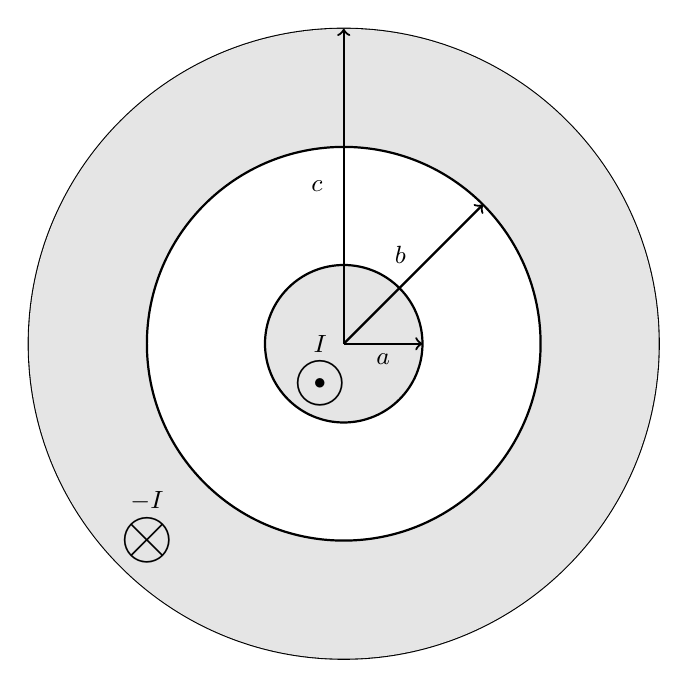
\begin{tikzpicture}
        % Definir los radios
        \def\ra{1}  % Radio interno
        \def\rb{2.5} % Radio intermedio
        \def\rc{4}  % Radio externo

        % Dibujar los círculos EXTERNOS primero
        \draw[thick] (0,0) circle (\rb);
        \draw[thick] (0,0) circle (\rc);

        % Sombreado de la región externa con líneas horizontales
        \begin{scope}
            \clip (0,0) circle (\rc);
            \fill[gray!20] (-5,-5) rectangle (5,5);
        \end{scope}


        % Eliminar el sombreado en la región entre a y b SIN BORRAR CONTORNOS
        \begin{scope}
            \clip (0,0) circle (\rb);
            \fill[white] (-5,-5) rectangle (5,5);
        \end{scope}
        \begin{scope}
            \clip (0,0) circle (\ra);
            \fill[gray!20] (-5,-5) rectangle (5,5);
        \end{scope}
        % Dibujar el círculo interno después para que su contorno sea visible
        \draw[thick] (0,0) circle (\ra);
        \draw[thick] (0,0) circle (\rb);

        % Flechas radiales
        \draw[thick,->] (0,0) -- (\ra,0) node[midway,below] {\small $a$};
        \draw[thick,->] (0,0) -- ({\rb*cos(45)},{\rb*sin(45)}) node[midway,above left,xshift=1pt] {\small $b$};
        \draw[thick,->] (0,0) -- ({\rc*cos(90)},{\rc*sin(90)}) node[midway,left,xshift=-4pt] {\small $c$};

        % Agregar símbolos de corriente
        \node at (-\ra+0.7,-\ra+0.5) {\Huge $\odot$};
        \node at (-\rc+1.5,-\rc+1.5) {\Huge $\otimes$};
        \node at (-\ra+0.7,-\ra+1) {\small $I$};
        \node at (-\rc+1.5,-\rc+2) {\small $-I$};

    \end{tikzpicture}
\end{center}
\end{problema}
\begin{proof} %Resolucion problema 2
    Laa resolucion viene dada por
    \begin{enumerate}
        \item Se busca obtener una expresión para la intensidad magnética \textbf{H} en todo el espacio. En base a la ley de Ampere se relaciona este con la densidad de corriente de la siguiente manera:
        \begin{equation}
            \oint_{C} H (\partial l) = \int\int_{S} J (\partial s) 
        \end{equation}
        Dado que la corriente es homogénea a lo largo de los medios luego podemos definir una densidad de carga superficial interna $J_{i}$ y una corriente superficial externa tal que $J_{e}$, tal que:
        \begin{equation}
            J_{i} = \frac{I}{\pi a^{2}}, \quad J_{e} = \frac{-I}{\pi (c^{2}-b^{2})}
        \end{equation}
        Luego se evaluará para las diferentes zonas de interés donde se utilizarán coordenadas cilíndricas dada la geometría del problema y dado que la corriente irá en ($\pm\hat{k}$), dada la regla de la mano derecha necesariamente ($\pm\hat{\theta}$) lo que será útil para definir los diferenciales:
        
        \subsubsection*{\underline{Zona 1} - \(0 \leq r \leq a\)}
        \begin{equation}
            \oint_C H (\partial l) = \int\int_{S} J (\partial S)
        \end{equation}
        \begin{equation}
            H(\rho)\int_{0}^{2\pi} \rho (\partial \theta) = J_{i} \int_{0}^{2\pi} \int_{0}^{\rho} \rho (\partial \rho )(\partial \theta )
        \end{equation}
        \begin{equation}
            H(\rho) 2\pi \rho = J_{i} \pi \rho^{2}
        \end{equation}
        \begin{equation}
            H(\rho) = J_{i} \frac{\rho}{2}
        \end{equation}
        \begin{equation}
            H(\rho) = \frac{I\rho}{2\pi a^{2}} \hat{\theta}
        \end{equation}
        
        \subsubsection*{ \underline{Zona 2} - $a \leq r \leq  b $}
        \begin{equation}
            \oint_C H (\partial l) = \int\int_{S} J (\partial S)
        \end{equation}
        \begin{equation}
             H(\rho)\int_{0}^{2\pi} \rho (\partial \theta) = I
        \end{equation}
        \begin{equation}
            H(\rho) = \frac{I}{2\pi \rho} \hat{\theta}
        \end{equation}
        
        \subsubsection*{ Zona 3 - $b\leq r \leq  c $}
        \begin{equation}
            \oint_C H (\partial l) =  \int\int_{S} J (\partial S)
        \end{equation}
        \begin{equation}
            H(\rho) 2\pi \rho = I + J_{e} \int_{0}^{2\pi} \int_{b}^{\rho} \rho (\partial \rho )(\partial \theta )
        \end{equation}
        \begin{equation}
             H(\rho) 2\pi \rho = I + J_{e} \pi (\rho^{2} - b^{2})
        \end{equation}
        \begin{equation}
              H(\rho) = \frac{I}{2\pi \rho} - \frac{I (\rho^{2} - b^{2})}{c^{2} - b^{2}}
        \end{equation}
        \begin{equation}
              H(\rho) = \frac{I(c^{2} - \rho^{2})}{2\pi \rho (c^{2} - b^{2})} \hat{\theta}
        \end{equation}
        
        \subsubsection*{ Zona 4 - $c\leq  r $}
        \begin{equation}
            \oint_C H (\partial l) =  \int\int_{S} J (\partial S)
        \end{equation}
        \begin{equation}
             H(\rho) 2\pi \rho = I-I
        \end{equation}
        \begin{equation}
            H(\rho) = 0
        \end{equation}
        Finalmente se calcula la intensidad H para las diferentes zonas para el cable coaxial.
        
        \item Se busca obtener el flujo magnético en el dieléctrico que viene caracterizado por $(\mu_{0},\epsilon)$, debemos considerar que el dieléctrico se encuentre en la zona 2, por lo que se tiene que el campo magnético \textbf{B} dependerá de $\rho$ tal que \textbf{B($\rho$}) relacionándose además con el valor obtenido para H en la zona 2 y recordando que $B = \mu H$. Por lo tanto el flujo magnético sobre una superficie vendrá dado por lo siguiente:
        \begin{equation}
            \phi = \int_{s} B(\rho)  (\partial S)
        \end{equation}
        \begin{equation}
                 = \int_{s} B(\rho) (\partial\rho)( \partial z) (\hat{\theta} \cdot \hat{\theta})
        \end{equation}
        \begin{equation}
                 = \frac{\mu I}{2\pi} \int_{0}^{l} \int_{a}^{b} \frac{1}{\rho} (\partial \rho)
        \end{equation}
        \begin{equation}
                 = \frac{\mu I \cdot l}{2\pi}\cdot ln\left(\frac{b}{a}\right)
        \end{equation}
        
        Por enunciado se menciona que se desea obtener la energía por unidad de largo, por lo que: 
        \begin{equation}
            \frac{W_{m}}{l}= \frac{\mu_{0} I^{2} ln(\frac{b}{a})}{4 \pi}
        \end{equation}
        Finalmente se obtiene la energía magnética por unidad de largo.
    \end{enumerate}
\end{proof}

\subsection{Problema}
\begin{problema}%Problema 3
    Para el dispositivo magnético de la figura 1.4 con dos material de permeabilidad $\mu_{1}$ y $\mu_{2}$, con espesores $d_{1}$ y $d_{2}$ y sección transversal circular de radio a, determinar: 
\begin{enumerate} 
    \item Potencial magnético escalar $\phi_{m}(z)$ en los medios 1 y 2, trabaje trabaje y campos $H_{1}$ y $H_{2}$ 
    \item Inductancia L del enrollado
    \item Energía magnética acumulada $W_{m}$ en los medios 1 y 2 
\end{enumerate}
\begin{center}
    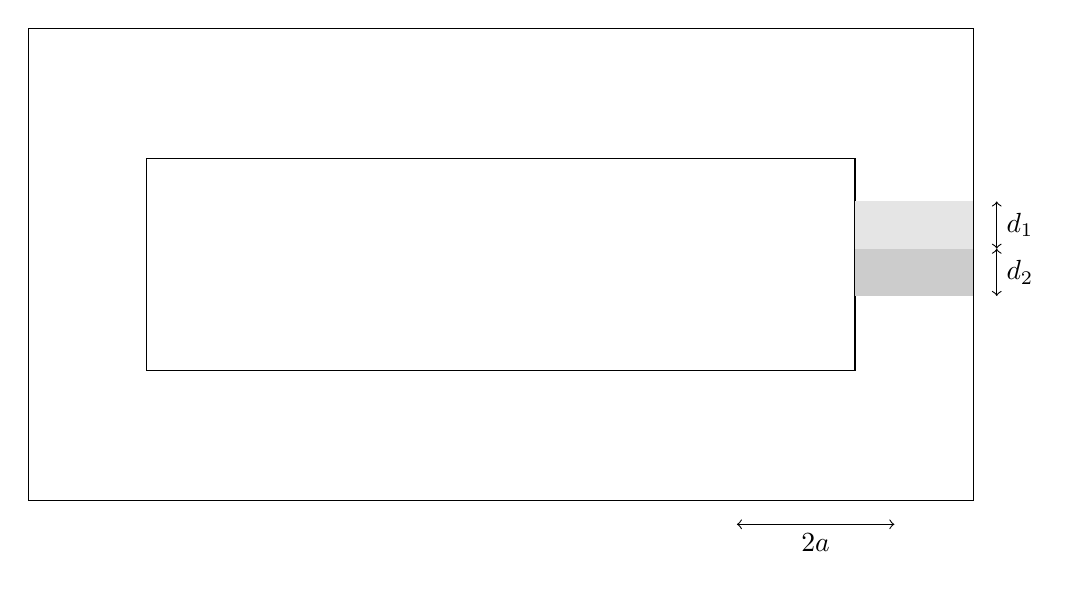
\begin{tikzpicture}
        % Dimensiones
        \def\a{1} % Aumentando la longitud horizontal
        \def\dOne{0.6}
        \def\dTwo{0.6}
        \def\coreWidth{6} % Reduciendo el ancho del núcleo ferromagnético
        \def\coreHeight{3}
        \def\gap{0.15} % Reduciendo el ancho del gap
        \def\offsetY{-0.4} % Ajuste para mover d1 y d2 más abajo
        \def\innerCoreWidth{9} % Haciendo el núcleo interno más ancho
    
        % Dibujar el núcleo
        \draw (-\coreWidth, -\coreHeight) rectangle (\coreWidth, \coreHeight);
        \draw (-\innerCoreWidth/2, -\coreHeight/2 + \gap) rectangle (\innerCoreWidth/2, \coreHeight/2 - \gap);
        
        % Dibujar la sección sombreada de d1
        \begin{scope}
            \clip (\innerCoreWidth/2, \offsetY+\dTwo) rectangle (\coreWidth, \offsetY+\dOne+\dTwo);
            \fill[gray!20] (\innerCoreWidth/2, \offsetY+\dTwo) rectangle (\coreWidth, \offsetY+\dOne+\dTwo);
        \end{scope}
        
        % Dibujar la sección sombreada de d2
        \begin{scope}
            \clip (\innerCoreWidth/2, \offsetY) rectangle (\coreWidth, \offsetY+\dTwo);
            \fill[gray!40] (\innerCoreWidth/2, \offsetY) rectangle (\coreWidth, \offsetY+\dTwo);
        \end{scope}
        
        % Etiquetas
        \draw[<->] (\coreWidth+0.3, \offsetY) -- ++(0, \dTwo) node[midway,right] {$d_2$};
        \draw[<->] (\coreWidth+0.3, \offsetY+\dTwo) -- ++(0, \dOne) node[midway,right] {$d_1$};
        \draw[<->] (\coreWidth/2, -\coreHeight-0.3) -- ++(2*\a, 0) node[midway,below] {$2a$};
        
    \end{tikzpicture}
\end{center}
\end{problema}

\begin{proof}%Resolucion problema 3
    La resolucion viene dada por:
   \begin{enumerate}
    \item Se busca obtener el potencial magnético escalar $\phi_{m}$, el cual es posible definirlo en condiciones de \textbf{flujo magnético nulo} principalmente y en otro tipo de condiciones. Este potencial se deberá obtener para los medios 1 y 2.
    
    \textit{Observación: No confundir con el potencial vector magnético A que se vio en el problema anterior, ni con el potencial escalar eléctrico $\phi_{e}$})

    Notemos que estamos en presencia de un núcleo ferromagnético (Muy usados en motores) que implicará una permeabilidad magnética casi infinita ($\mu \rightarrow \infty$). Además, en el núcleo ferromagnético tenemos lo siguiente con relación con respecto a la intensidad magnética: 
    \begin{align}
        H = \frac{1}{\mu} B 
    \end{align}
    Dada la consideración anterior se tendrá que $H \rightarrow 0 $, es de importancia considerar que esta relación la podemos realizar dado que no estamos en presencia de un desplazamiento eléctrico variable en el tiempo $\textbf{D}$ (ver ecuaciones de Maxwell). Debido a lo anterior, no se tendrá una corriente superficial en el núcleo: 
    \begin{align}
        \nabla \times H = J  
    \end{align}
    Siendo de esta manera consistente, se tendrá: 
    \begin{align}
        \nabla \times H = 0  
    \end{align}
    De esta manera similar al campo vectorial eléctrico se podrá definir un potencial escalar para la intensidad de campo magnético $H$ tal que:
    \begin{equation}
        H = -\nabla \phi_{m} 
    \end{equation}
    En base a esto podemos verificar de manera directa que cumple con la ecuación de Laplace:\\
    \begin{align}
        \nabla \cdot B = \nabla \cdot \mu H= 0 
    \end{align}
    Lo cual es equivalente a 
    \begin{align}
        \nabla \cdot H &= 0\\
        \nabla \cdot (-\nabla \phi_{m}) &= 0\\
        \nabla^{2} \phi_{m}= 0 
    \end{align}
    Con lo que finalmente se logra definir un potencial magnético. Luego podemos analizar el tipo de coordenadas a utilizar, se observa que es de conveniencia el utilizar coordenadas cilíndricas, con lo que:
    \begin{align}
        \nabla^{2}\phi_{m} = \frac{1}{\rho} \frac{d}{d\rho}\left(\rho \frac{d\phi}{d\rho}\right) + \frac{1}{\rho^{2}}\frac{d^{2}\phi}{d\rho^{2}} + \frac{d^{2}\rho}{dz^{2}}
    \end{align}
    Se tendrá que el potencial escalar magnético dependerá de una sola dirección, es decir, $\phi_{m}(z)$ por tanto:
    \begin{align}
        \nabla^{2} \phi(z) = \frac{d^{2} \phi_{m}}{dz^{2}} &= 0\\
        \frac{d^{2} \phi_{m}}{dz^{2}} &= 0\\
        \frac{d\phi_{m}}{dz} &= A\\
        \phi_{m}(z) &= Az + B
    \end{align}
    Se obtiene la forma del campo magnético escalar. Luego tenemos la presencia de dos medios, por lo tanto deberemos hacer la distinción entre cada uno de estos.
    \begin{align}
        \phi_{m1}(z) &= Az + B \\
        \phi_{m2}(z) &= Cz + D 
    \end{align}
    Con lo que de manera análoga se deberá encontrar 4 ecuaciones tal que permitan despejar estas constantes. Usando las condiciones de borde entregadas.
    \subsubsection*{\underline{Medio 1}}
    \begin{align}
        \phi_{m1}(z=(d_{1} + d_{2}))  &= A(d_{1} + d_{2}) + B \\&= N I_{0} 
    \end{align}
    \subsubsection*{\underline{Medio 2}}
    \begin{align}
        \phi_{m2}(z=0)  &= C\cdot 0+ D \\&= 0
    \end{align}
    Lo que implicará de manera directa que $D=0$. Se tendrá además que el campo magnético escalar deberá ser continuo.
    \begin{align}
        \phi_{m1}(z=d_{2}) &=\phi_{m2}(z=d_{2}) \\ A d_{2} + B &= C d_{2} 
    \end{align}
    Dado que se busca el obtener otra ecuación, se deriva de lo siguiente:
    \begin{align}
        H_{1} &= - \nabla \phi_{m1} &  
        H_{2} &= - \nabla \phi_{m2}\\
         H_{1}&= -\frac{d\phi_{m1}}{dz} &   H_{2}&= -\frac{d\phi_{m2}}{dz}\\
         &= -A  &  &= -C
    \end{align}
    De esta manera tenemos que por condición de borde y dado que el campo tiene solo componente normal en la zona de interés se cumple:
    \begin{align}
        B_{1n} &= B_{2n}\\
        \mu_{1}H_{1} &=  \mu_{2}H_{2}\\
        \mu_{1}A &=  \mu_{2}C   
    \end{align}
    Luego se puede plantear 4 set de ecuaciones las cuales vendrán dados:
    \begin{align}
        NI_{0} &= A(d_{1} + d_{2}) + B\\
        D&=0\\
        \mu_{1}A &=  \mu_{2}C\\
        Ad_{2} + B &= Cd_{2}
    \end{align}
    Luego despejando las variables se obtiene lo siguiente:
    \begin{align}
    A &= \frac{\mu_{2} N I_{0}}{d_{2}(\mu_{1} + \mu_{2})}\\
     B&= \left(\frac{NI_{0}\mu_{1}}{d_{2}(\mu_{1} + \mu_{2})}\right) d_{2} - \left(\frac{\mu_{2} N I_{0}}{d_{2}(\mu_{1} + \mu_{2})}\right)d_{1}\\
     C&= \frac{NI_{0}\mu_{1}}{d_{2}(\mu_{1} + \mu_{2})}\\
     D&=0
    \end{align}
    Finalmente se despejan que permiten el determinar tanto $H_{1} , H_{2},\phi_{m1}$  y $\phi_{m2} $.
    \item Se busca obtener la inductancia L que vendrá caracterizada por la siguiente expresión: 
    \begin{align}
        L = \frac{\phi N}{I}
    \end{align}
    Donde $\phi$ corresponde al flujo magnético y nos da una idea de cuando campo magnético hay en una superficie dada y deberá por tanto, considerar ambos medios:
    \begin{align}
        \phi_{1} &= \int B_{1} dS\\
                 &= \mu_{1} \int_{S} H_{1} dS\\
                 &= \mu_{1} \int_{0}^{2\pi} \int_{0}^{a} A (-\hat{z}) \cdot r (dr) (d\theta) (-\hat{z})  \\
                 &= \mu_{1}  \pi a^{2} A\\
                 &= \mu_{1}\pi a^{2} \left(\frac{\mu_{2} N I_{0}}{d_{2}(\mu_{1} + \mu_{2})}\right)
      \end{align}
    De manera análoga tenemos que el flujo para la otra superficie vendrá dado por:
    \begin{align}
        \phi_{2} &= \int B_{2} dS\\
                 &= \mu_{2} \int_{S} H_{2} dS\\
                 &= \mu_{2} \int_{0}^{2\pi} \int_{0}^{a} C (-\hat{z}) \cdot r (dr) (d\theta) (-\hat{z})  \\
                 &= \mu_{2}  \pi a^{2} C\\
                 &= \mu_{2}\pi a^{2} \left(\frac{\mu_{1} N I_{0}}{d_{2}(\mu_{1} + \mu_{2})}\right)
      \end{align}
    Una vez obtenido el flujo magnético para ambos medios se logra obtener la inductancia utilizando la expresión:
    \begin{align}
        L = \frac{\phi N}{I_{0}}
    \end{align}
    \textit{Observación: Es importante considerar que es posible tomar cualquier flujo para calcular la inductancia, esto debido a que por condiciones de borde se tendrá que $B_{1} = B_{2}$ y por tanto el utilizar una u otra es análogo.}
    \item Debemos obtener la energía magnética acumulada $W_{m}$ en ambos medios, para esto se utilizará la siguiente expresión:
    \begin{align}
        w_{m} = \frac{1}{2} \mu H^{2}
    \end{align}
    Luego como se quiere la energía magnética se integra sobre un volumen tal que:\\
    \subsubsection*{\underline{Medio 1}}
    \begin{align}
        W_{m1} &= \frac{\mu_{1}}{2}\int_{v} H_{1}^{2} dv\\
               &= \frac{\mu_{1}}{2}A^{2} \int_{d2}^{d1+d2} \int_{0}^{2\pi} \int_{0}^{a} r (dr) (d\theta) (dz)\\
               &=\frac{\mu_{1}}{2} A^{2} \pi a^{2}d_{2} 
    \end{align}
    \subsubsection*{\underline{Medio 2}}
    \begin{align}
        W_{mw} &= \frac{\mu_{w}}{2}\int_{v} H_{2}^{2} dv\\
               &= \frac{\mu_{2}}{2}C^{2} \int_{0}^{d1} \int_{0}^{2\pi} \int_{0}^{a} r (dr) (d\theta) (dz)\\
               &=\frac{\mu_{2}}{2} C^{2} \pi a^{2}d_{1} 
    \end{align}
    Finalmente se obtienen las energías acumuladas en los dos diferentes medios dado que A y C son términos conocidos.
\end{enumerate}

\end{proof}

\subsection{Problema} %Problema 4
\begin{problema}
    Una densidad $\mathbb{J} = J_{0} \hat{{z}}$ origina un potencial magnético vectorial:
\begin{align}
    \textbf{A}= \frac{-\mu_{0}J_{0}}{4}(x^{2}+y^{2})\hat{z}
\end{align}
\begin{enumerate}
    \item Use la ecuación de Poisson vectorial para comprobar el enunciado 
    \item Mediante \textbf{A} calcule el campo magnético \textbf{B}.
    \item Utilice \textbf{J} y la ley de Ampere para calcular nuevamente \textbf{B}, compare los resultados.
\end{enumerate}
\begin{center}
    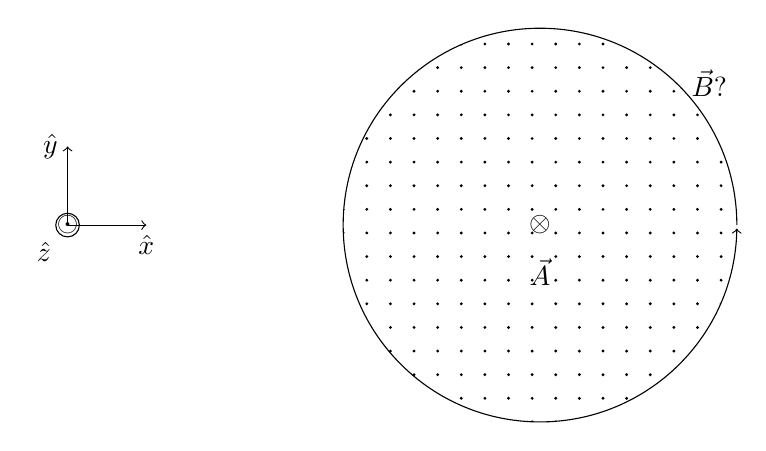
\begin{tikzpicture}[scale=1] % Aumentando el tamaño
        % Sistema de coordenadas desplazado a la izquierda
        \draw[->] (-3,0) -- (-2,0) node[below] {$\hat{x}$};
        \draw[->] (-3,0) -- (-3,1) node[left] {$\hat{y}$};
      
        \draw (-3,0) circle (0.15);
        \draw (-3,0) node {$\odot$};
        \node[below] at (-3.3,-0.1) {$\hat{z}$};
        % Círculo con puntos dentro y flecha en el contorno
        \begin{scope}
            \clip (3,0) circle (2.5); % Tamaño aumentado
            \foreach \x in {0.5,0.8,...,5.5} {
                \foreach \y in {-2.5,-2.2,...,2.5} {
                    \fill[black] (\x,\y) circle (0.02);
                }
            }
        \end{scope}
        
        % Contorno con flecha
        \draw[->] (5.5,0) arc (0:359:2.5); % Tamaño aumentado
        
        % Vector A
        \node at (3,0) {$\otimes$};
        \node[below] at (3,-0.3) {$\vec{A}$};
        
        % Etiqueta B
        \node[right] at (4.8,1.8) {$\vec{B} ?$};
    
    \end{tikzpicture}
\end{center}
\end{problema}
\begin{proof} %Resolucion problema 4
    La resolucion viene dada por:
    \begin{enumerate}
        \item Sea una densidad de corriente \textbf{J} = $J_0 \hat{z}$, el cual originará un potencial magnético. Este último se produce debido a las relaciones entre las ecuaciones de Maxwell y al hecho de que $\nabla \cdot B = 0$, permitiendo que $B = \nabla \times A$. Retomando la resolución, este campo A se caracteriza por:
            \begin{equation}
                A = \frac{-\mu_0 J_0}{4}(x^2 + y^2) \hat{z}
            \end{equation}
            Se comprobará que \textbf{A} sea el potencial de \textbf{J}, mediante la siguiente relación:
            \begin{equation}
                \nabla^2 A = -\mu_0 J_0
            \end{equation}
            Realizando el análisis por componente, se observa que el campo vectorial A tiene componentes solo en $\hat{z}$:
            \begin{align}
                \nabla^2 A_x &= -\mu_0 J_x = 0, \\
                \nabla^2 A_y &= -\mu_0 J_y = 0, \\
                \nabla^2 A_z &= -\mu_0 J_z = -\mu_0 J_0.
            \end{align}
            Calculando $\nabla^2 A$, tenemos que:
            \begin{equation}
                \begin{aligned}
                    \nabla^2 A &= \frac{\partial^2 A}{\partial x^2} + \frac{\partial^2 A}{\partial y^2} + \frac{\partial^2 A}{\partial z^2} \\
                               &= \frac{-\mu_0 J_0}{2} + \frac{-\mu_0 J_0}{2} + 0 \\
                               &= -\mu_0 J_0
                \end{aligned}
            \end{equation}
            
            Por tanto se comprueba que el campo vectorial A es el potencial de J.
        \item En base a lo anterior se busca obtener el campo magnético \(B\) mediante \(A\):
            \begin{equation}
                B = \nabla \times A
            \end{equation}
            Se obtendrá la expresión explícita para el rotor de \(A\):
            \begin{equation}
                \nabla \times A = \begin{bmatrix} \hat{x} & \hat{y} & \hat{z} \\ \frac{\partial}{\partial x} & \frac{\partial}{\partial y} & \frac{\partial}{\partial z} \\ 0 & 0 & A \end{bmatrix}
            \end{equation}
            Luego resolviendo dicho rotor, se obtiene:
            \begin{equation}
                \nabla \times A = \frac{\partial A}{\partial y} \hat{x} - \frac{\partial A}{\partial x} \hat{y} = \frac{-\mu_0 J_0}{2}(y \hat{x} - x \hat{y})
            \end{equation}
        \item Se busca obtener \textbf{B} mediante la ley de Ampere, la cual se obtiene mediante la siguiente relación:
            \begin{equation}
                \oint_C B \, d\ell = \int_S J \, dS = I_{\text{encerrada}}
            \end{equation}
            Dada la geometría del sistema, se utiliza una circunferencia de radio r. Despejando el término \textbf{B} dado que no depende de la geometría del sistema para términos de la integral:
            \begin{align}
                \oint_C B \, d\ell &= \mu_0 J_0 \int_{0}^{2\pi} \int_{0}^{r} \rho \, d\rho \, d\theta, \\
                B (2\pi r) &= \mu_0 J_0 \pi r^2, \\
                B &= \frac{\mu_0 J_0 r}{2} \hat{\phi}.
            \end{align}
            Realizando el cambio a coordenadas cilíndricas:
            \begin{equation}
                B = \frac{-\mu_0 J_0}{2}(y\hat{x} - x\hat{y}) = \frac{-\mu_0 J_0 \rho}{2}(\sin(\phi) \hat{x} - \cos(\phi) \hat{y}) = \frac{-\mu_0 J_0 \rho}{2} \hat{\phi}
            \end{equation}
    \end{enumerate}  
\end{proof}